\section{Marco conceptual}

\subsection{API}
\textit{Application Program Interface} por sus siglas en inglés, es código que actúa como interfaz para la programación de aplicaciones, permitiendo por ejemplo, que dos aplicaciones se comuniquen entre si, como el acceder a funcionalidades sin la necesidad de conocer la complejidad del código implementado \citep{techtarget-API}. Por ejemplo, para el sistema operativo \footnote{En resumidas palabras, un sistema operativo (OS por sus siglas en inglés) es un software que, después de ser cargado en la computadora por un programa de arranque inicial, administra los recursos de una computadora, controlando el flujo de información hacia y desde un procesador principal, administrando recursos como, la memoria, redes, archivos, etc. \citep{gartner-group-OS}} Android, todo su conjunto de funciones está disponible mediante APIs escritas en el lenguaje Java. Estas APIs son los cimientos necesarios para crear aplicaciones de Android simplificando la reutilización de componentes del sistema, servicios centrales y modulares.

\subsection{SDK}
Es un conjunto de utilidades de desarrollo para escribir aplicaciones de software, generalmente asociadas a entornos específicos \citep{gartner-group-SDK}. Ejemplos de SDKs incluyen a Windows 7 SDK, the Mac OS X SDK, iPhone SDK y Android SDK. 

Los SDK suelen incluir un entorno de desarrollo integrado (IDE), que sirve como interfaz de programación central. El IDE puede incluir una ventana de programación para escribir el código fuente, un depurador para corregir errores del programa y un editor visual, que permite a los desarrolladores crear y editar la interfaz gráfica de usuario (GUI) del programa. Los IDE también incluyen un compilador, que se usa para crear aplicaciones a partir de archivos de código fuente \citep{techterms-SDK}.

La mayoría de los SDK contienen código de ejemplo, que proporciona a los desarrolladores ejemplos de programas y bibliotecas. Estas muestras ayudan a los desarrolladores a aprender cómo crear programas básicos con el SDK, lo que les permite eventualmente crear aplicaciones más complejas. Los SDK también ofrecen documentación técnica, que puede incluir tutoriales y preguntas frecuentes. Algunos SDK también pueden incluir gráficos de muestra, como botones e iconos, que se pueden incorporar a las aplicaciones \citep{techterms-SDK}. En resumen, un SDK usualmente incluye lo siguiente:

\begin{itemize}
\item APIs
\item IDE
\item Software de configuración
\item Códigos de ejemplo (programas, pruebas de concepto y bibliotecas)
\item Documentación (técnica, tutoriales, preguntas frecuentes)
\item Materiales gráficos de muestra (iconos, botones, etc.)
\end{itemize}



%\subsection{Haptics}
% http://www.scielo.org.co/scielo.php?script=sci_arttext&pid=S1794-12372016000200002
%Haptics es una tecnología táctil o de retroalimentación de fuerza que aprovecha el sentido del tacto de una persona al aplicar vibraciones y / o movimiento a la punta del dedo del usuario. Esta estimulación puede ayudar a la tecnología en el desarrollo de objetos virtuales en la pantalla del dispositivo. En su sentido más amplio, hápticos puede ser cualquier sistema que incorpore elementos táctiles y vibre a través de un sentido del tacto \citep{gartner-group-haptics}. OpenGlove posee

\subsection{Tipos de aplicaciones móviles}
Actualmente los sistemas operativos que predominan el mercado de dispositivos móviles son dos, iOS con un 14.4\% y Android con un 84,8\%  \citep{statista-SO-war-mobile}. Cuando se habla de desarrollar aplicaciones móviles se tienen como objetivo los dispositivos que tienen iOS o Android como sistema operativo. A continuación se detallan los tres principales tipos de aplicaciones móviles: Nativas, Híbridas y Web.

%https://www.solbyte.com/blog/2014/07/21/tipos-de-aplicaciones-moviles-nativas-webs-hibridas/

%https://clearbridgemobile.com/mobile-app-development-native-vs-web-vs-hybrid/

% Very interesant : https://www.mobiloud.com/blog/native-web-or-hybrid-apps/

	\subsubsection{Nativas}
	Apple y Google ofrecen a los desarrolladores de aplicaciones sus propias herramientas de desarrollo, elementos de interfaz y SDK estandarizado; Xcode y Android Studio. Esto permite a cualquier desarrollador profesional desarrollar una aplicación nativa con relativa facilidad.
	
	Las ventajas que ofrecen las aplicaciones móbiles nativas, son mayor rapidez que las aplicaciones Híbridas y Web, también una experiencia con elementos de interfaz nativos. Con aplicaciones nativas, es posible acceder a la cámara, el micrófono, almacenamiento interno, Bluetooth, la brújula, el acelerómetro y deslizar gestos fácilmente. Todavía es posible usar las alternativas, pero es más directo de manera nativa \citep{mobile-apps-types}.
	
	Las desventajas de las aplicaciones nativas es que se requiere más de un código base, dado que las aplicaciones iOS no se ejecutarán en Android y viceversa, por lo que se tiene que trabajar con diferentes códigos para cada plataforma que se elija construir. Esto se traduce a mayores costos de mantención, puesto que se  necesitan desarrolladores con conocimientos en ambas plataformas o bien equipos diferenciados, teniendo ambos que desarrollar lo mismo en ambas aplicaciones nativas \citep{mobile-apps-types}.

Actualmente existen alternativas a las herramientas para desarrollo nativo ofrecidas por iOS y Android. Estas son, Xamarin, React Native y Titanum, las cuales permiten desarrollar aplicaciones nativas multiplataforma (cross-platform) para iOS y Android. Gracias a estas alternativas se permite compartir código para ambas plataformas. 
	
	\subsubsection{Web}
	La mayoría están desarrolladas en JavaScript, CSS y HTML5. No poseen SDK para trabajar con iOS y Android. En resumidas cuentas son aplicaciones web que son adaptadas para parecer aplicaciones nativas, pero sin acceder completamente a las funcionalidades del dispositivo y sin tener un comportamiento igual al nativo. 
	
	Hasta hace poco, las aplicaciones web carecían de la funcionalidad de las aplicaciones nativas, como la capacidad de enviar notificaciones automáticas, trabajar sin conexión y cargar en la pantalla de inicio.

Sin embargo, han habido algunas mejoras en los navegadores y aplicaciones web que ofrecen estas características. Las aplicaciones que aprovechan estas características se denominan aplicaciones web progresivas \citep{mobile-apps-types}. Esta alternativa permite compartir el 100\% del código para ambas plataformas, ya que son aplicaciones web accedidas por Internet desarrolladas con herramientas web.
	
	\subsubsection{Híbridas}
	Se instala como una aplicación nativa, pero en realidad es una aplicación web en el interior. Las aplicaciones híbridas, como las aplicaciones web, se crean con Javascript, HTML y CSS y se ejecutan en algo llamado Webview, un navegador simplificado dentro de su aplicación.
	Las ventajas que presentan estas aplicaciones es que son menos costosas ya que comparten el mismo código base. Al igual que con las aplicaciones nativas, conserva la misma capacidad para acceder a las funciones del dispositivo. Esto es gracias a soluciones como PhoneGap que actúan como un puente entre el SDK nativo y la vista web en la que se ejecuta la aplicación. 
	
	La principal desventaja de este tipo de aplicación móvil, es su rendimiento, además de que presentan diferencias en el comportamiento respecto de las aplicaciones nativas. Algunas de las alternativas existentes para desarrollar aplicaciones híbridas son: PhoneGap/Cordova y Canvas. \citep{mobile-apps-types}

\subsection{WebSocket}
WebSocket es un protocolo que provee un canal de comunicación bidireccional y simultáneo (full-duplex) entre un cliente y un servidor, utilizando un único socket TCP \footnote{TCP: es un protocolo que cubre las capa de transporte del modelo de red de siete capas OSI (Open System Interconnection) \url{https://www.gartner.com/it-glossary/tcpip-transmission-control-protocolinternet-protocol}} (Transmission Control Protocol). Este protocolo inicia un HandShake, el cual consiste en un request HTTP\footnote{HTTP (Hypertext Transfer Protocol): es una capa del nivel de aplicación para transmitir documentos de hipermedia (del inglés hypermedia) como lo es un documento HTML} para establecer la conexión entre el cliente y servidor \citep{websocket-html5} . Esta petición establece el upgrade del protocolo HTTP al de WebSocket. Por tanto el protocolo HTTP solo se utiliza para establecer una conexión persistente mediante un socket TCP, el cual permite el intercambio de mensajes full-duplex mientras el socket sea cerrado por alguna de las partes. El servidor puede mantener múltiples clientes conectados, intercambiando mensajes de manera simultánea, permitiendo el desarrollo de aplicaciones que requieren interacción en tiempo real, como por ejemplo, los juegos en línea o gráficas en tiempo real para el mercado de las divisas (Currency Market) \citep{websocket-scalability}. La Figura \ref{fig:WebSocket} muestra la representación visual del protocolo WebSocket anteriormente explicado.

\begin{figure}[H]
  \begin{center} 
   	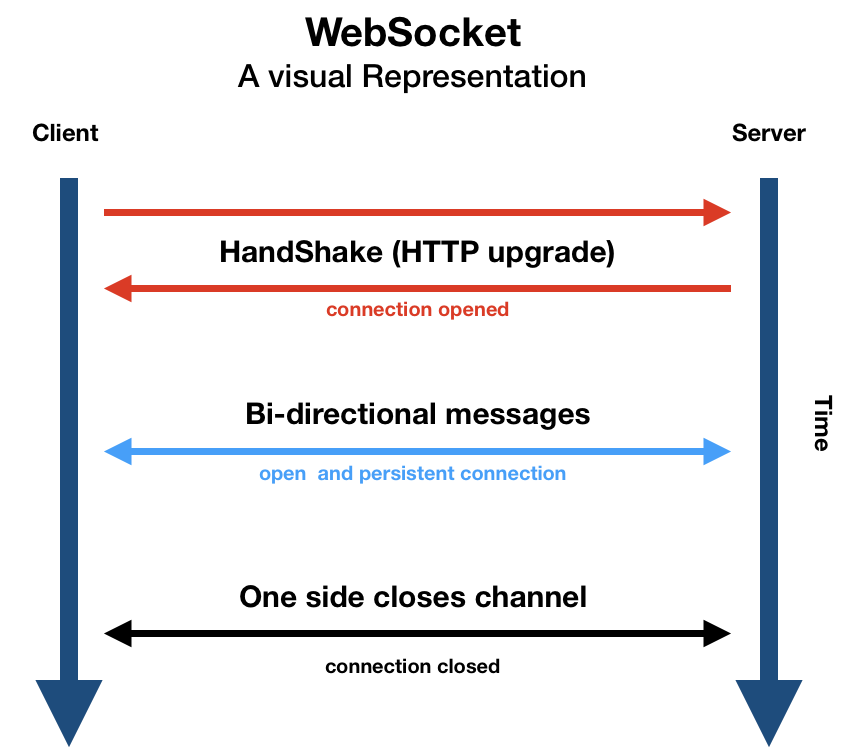
\includegraphics[width=0.5\textwidth]{images/chapter02/websockets-guides-transparent.png} 
    \caption[Representación visual de WebSocket]{Representación visual de WebSocket \\Fuente: \cite{websocket-pubnub}} 
    \label{fig:WebSocket}
  \end{center}
\end{figure}

Para un mayor entendimiento sobre WebSocket es necesario citar la publicación de \cite{websocket-oreilly}. En el capítulo 17 define lo siguiente: "WebSocket es un conjunto de múltiples estándares: WebSocket API\footnote{WebSocket API estándar: \url{https://html.spec.whatwg.org/multipage/web-sockets.html}} que es definida por la W3C y el protocolo WebSocket (RF 6455\footnote{Protocolo estándar WebSocket: \url{https://tools.ietf.org/html/rfc6455} }) cuyas extensiones son definidas por HyBi Working Group (IETF)". En definitiva para hacer uso del protocolo se hace uso de la API  WebSocket, permitiendo abstraer la complejidad detrás del protocolo, el cual es establecido bajo el estándar RF 6455.

La API de WebSocket es simple de usar, esto se puede observar los siguientes eventos presentes en clientes y servidores WebSocket:

\begin{itemize}
		\item \textbf{On Open:} Este evento se activa cuando cuando se ha abierto una nuevo socket.
		\item \textbf{On Message:} Este evento se activa cuando se recibe un nuevo mensaje.
		\item \textbf{On Error:} Este evento se activa cuando ocurre un error en la conexión WebSocket.
		\item \textbf{On Close: }Este evento se activa cuando ocurre cuando el socket es cerrado por el cliente o el servidor. 
\end{itemize}



%\citep{websocket-html5}
%\citep{websocket-scalability}
%\citep{websocket-oreilly}

